\chapter{Implementation}

\section{Implementation Overview}
Implementation was carried out in Python using a modular project structure. The workflow covers dataset preparation, model training, evaluation, and result visualization.

\section{Development Environment}
\begin{itemize}
\item Language: Python 3.8+
\item Deep Learning Framework: PyTorch
\item Supporting Libraries: TorchVision, NumPy, scikit-learn, Matplotlib
\item Interface Framework: Gradio (for demo)
\end{itemize}

\section{Code Organization}
Core implementation modules are organized as follows:
\begin{itemize}
\item \texttt{src/data/prepare\_dataset.py}: category mapping and split preparation
\item \texttt{src/models/model.py}: architecture definitions
\item \texttt{src/models/train.py} and \texttt{src/models/train\_advanced.py}: training logic
\item \texttt{src/evaluation/evaluate.py}: metric computation and evaluation pipeline
\item \texttt{run\_training.py}: project-level training entry point
\item \texttt{demo\_app.py}: interactive inference demo
\end{itemize}

\section{Recent Script-Level Updates Incorporated}
The latest project updates include advanced model training utilities in \path{src/models/train_advanced.py}. These additions provide:
\begin{itemize}
\item dedicated training configurations for EfficientNet-B0 and ViT-B/16,
\item warmup-cosine learning-rate schedules,
\item gradient clipping support for transformer stability,
\item label smoothing and AdamW-based optimization,
\item resumable checkpointing with optimizer/scheduler states.
\end{itemize}

The model factory in \texttt{src/models/model.py} now supports ResNet-50, EfficientNet-B0, and ViT creation through a unified API, enabling controlled architecture comparison in Semester 2.

\section{Data Pipeline Implementation}
The preprocessing pipeline loads images from class folders, applies transformation sequences, and creates dataloaders for train, validation, and test stages. Split statistics are recorded to support repeatable experiments.

Operationally, this pipeline includes deterministic ordering and split metadata persistence to minimize accidental leakage across training and evaluation sets. During debugging, this design enables direct traceability from a metric anomaly back to dataset partition and transformation stage.

\section{Training Implementation}
The training loop performs forward pass, loss computation, backpropagation, and optimizer updates per mini-batch. For each epoch, aggregate loss and accuracy are logged for both training and validation sets. Model checkpointing preserves the best-performing weights.

The implementation also supports controlled extension to advanced architectures through a shared trainer interface. This reduces duplication and ensures that comparison runs differ in model/hyperparameters rather than hidden infrastructure behavior.

\section{Logged Training Behavior}
The available training history indicates steady convergence over 15 epochs:
\begin{itemize}
\item Training loss decreased from 0.7835 to 0.6069.
\item Validation loss decreased from 0.7296 to 0.5758.
\item Validation accuracy improved from 72.95\% to 79.17\% during training phase.
\end{itemize}

These trends support stable optimization before final test evaluation.

\section{Evaluation Implementation}
The evaluation module computes confusion matrix and macro metrics from model predictions. Results are exported as JSON for traceability and plotted using standardized visualization scripts.

In addition, helper routines provide misclassification extraction with confidence context, enabling targeted review of high-confidence failures. This is particularly useful for debugging boundary classes before extending the system to exact-location inference.

\begin{figure}[htbp]
\centering
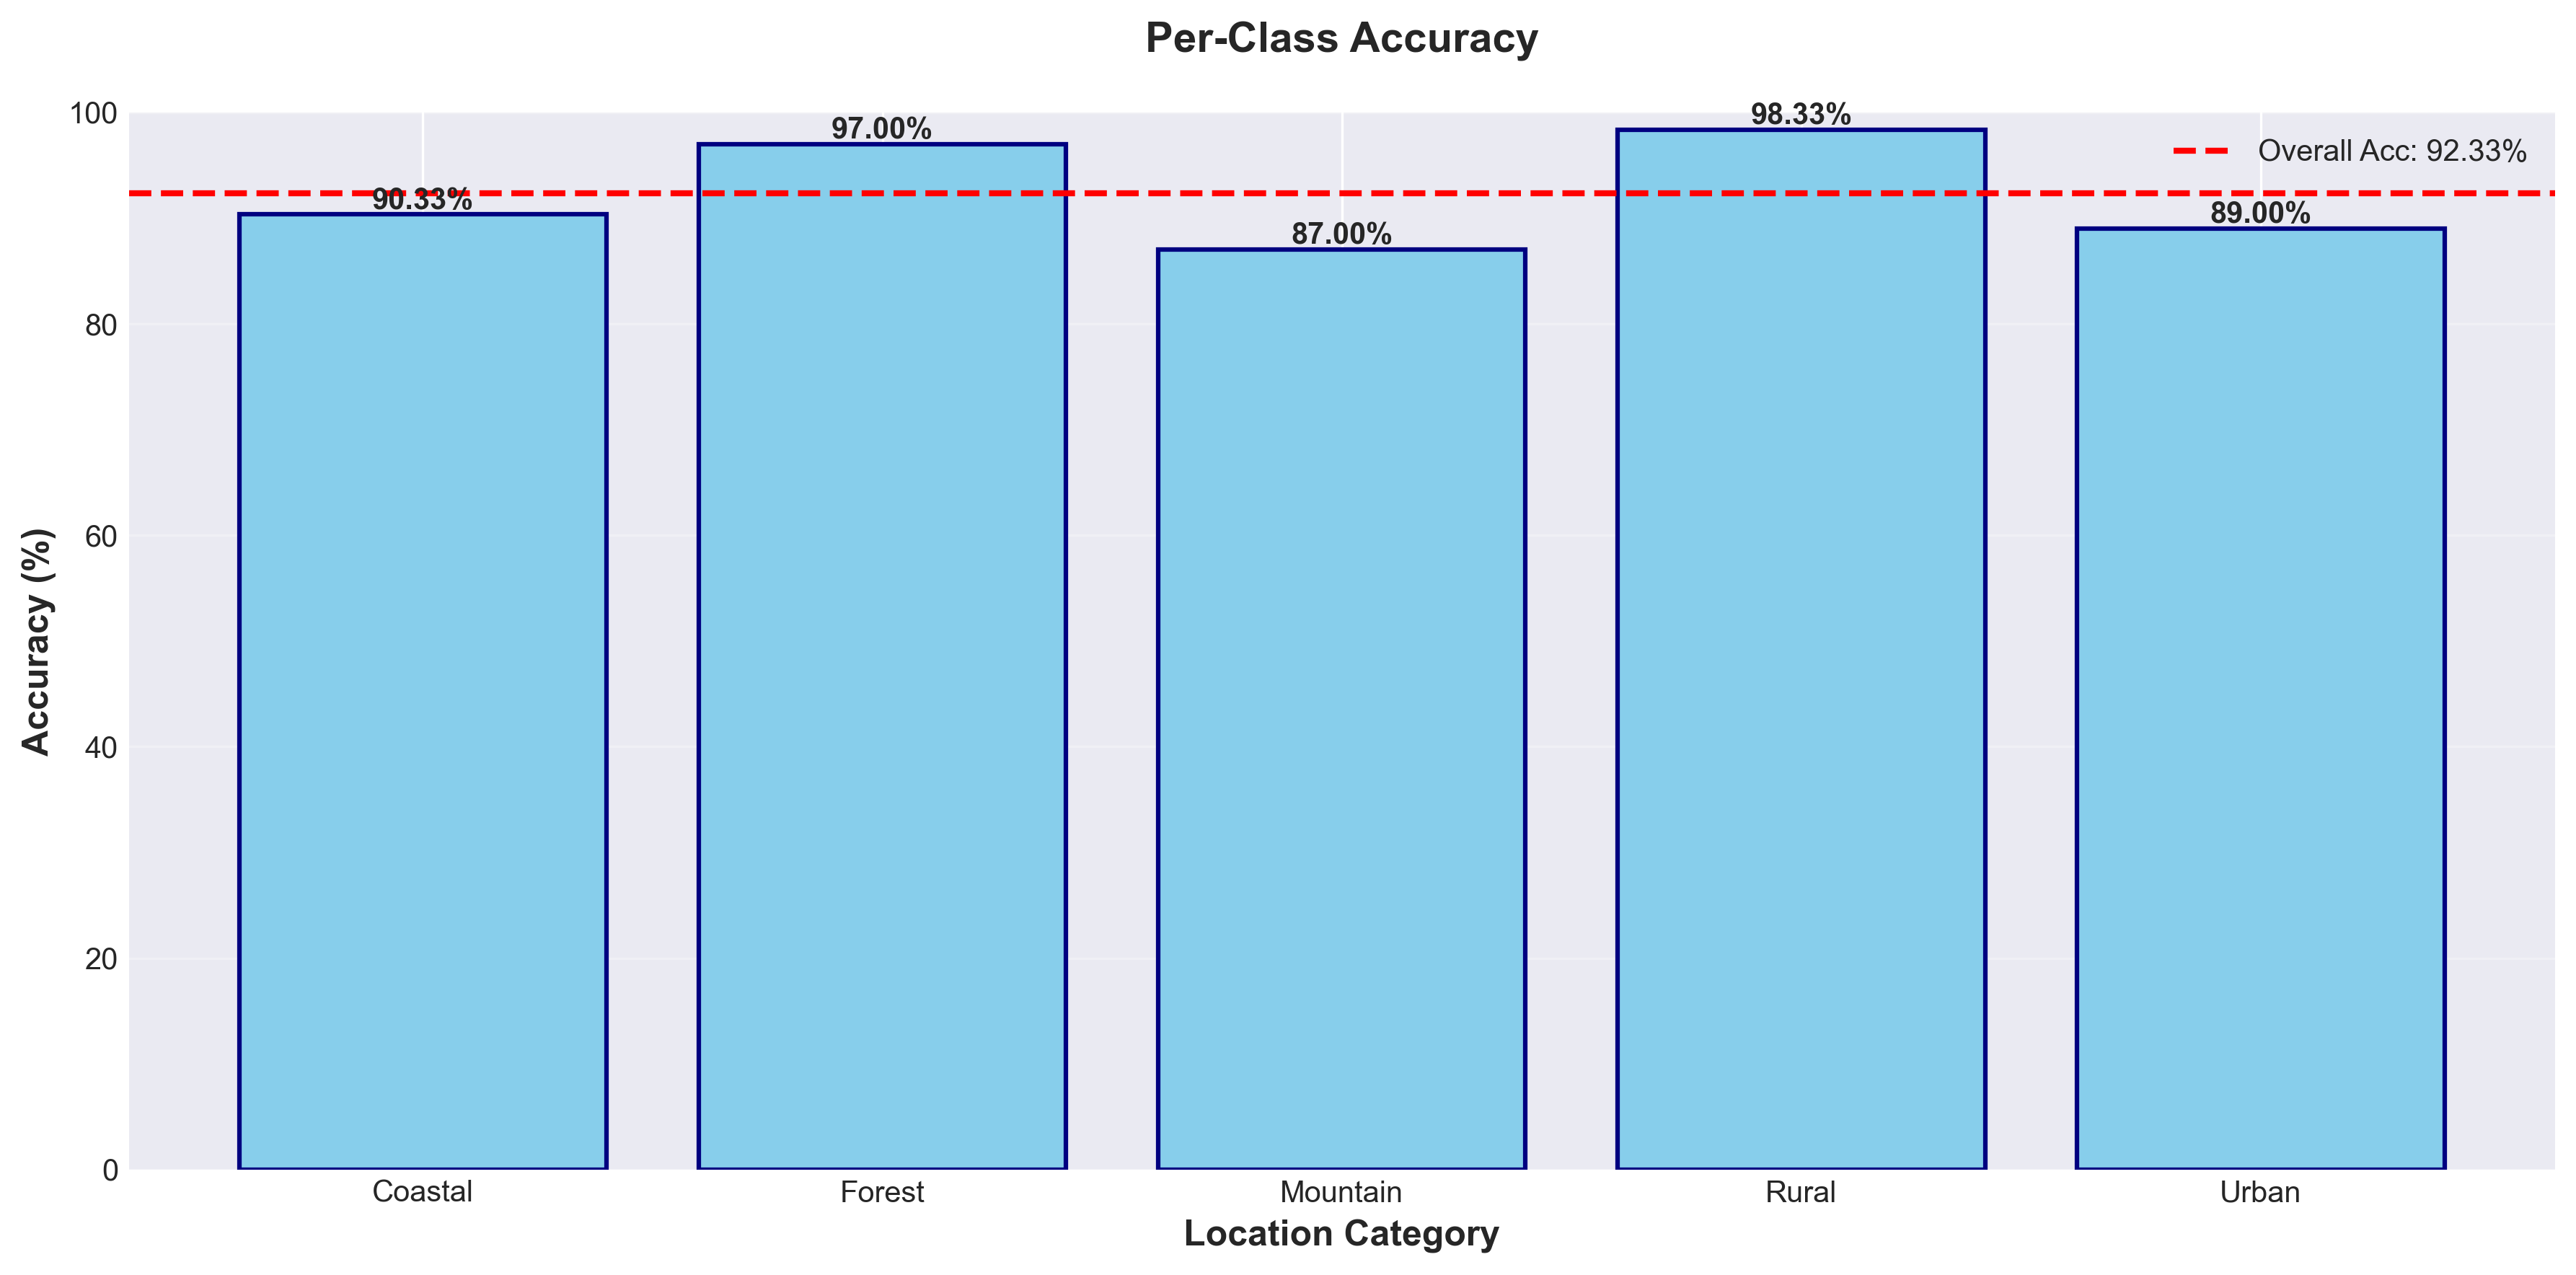
\includegraphics[width=0.80\textwidth]{assets/figures/per_class_accuracy.png}
\caption{Per-class accuracy generated by evaluation scripts}
\label{fig:perclass-impl}
\end{figure}

\begin{figure}[htbp]
\centering
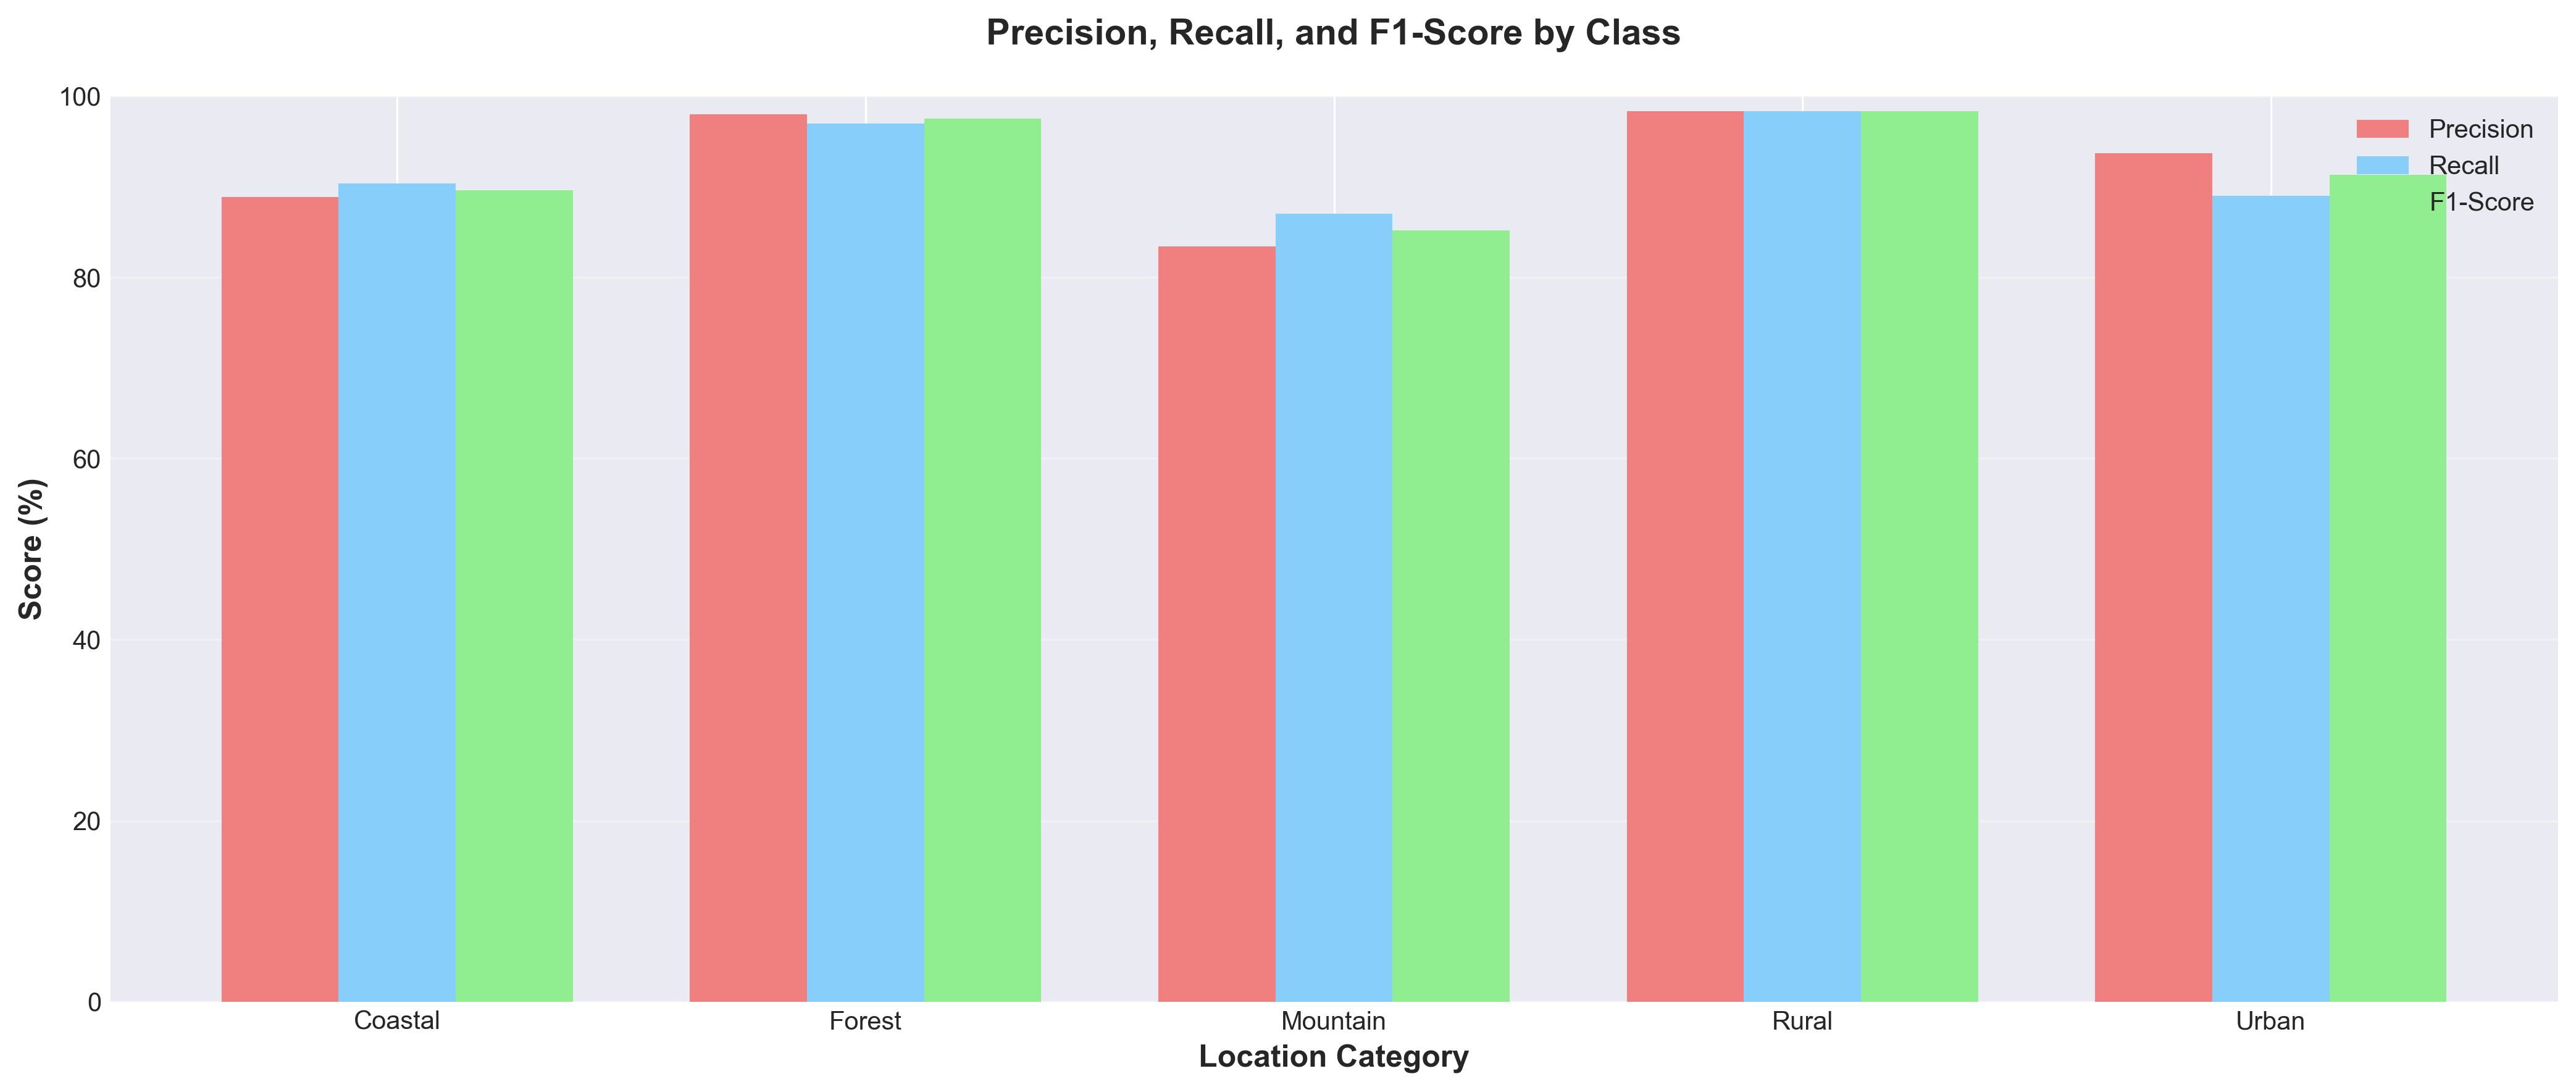
\includegraphics[width=0.80\textwidth]{assets/figures/metrics_comparison.png}
\caption{Comparison of aggregate evaluation metrics}
\label{fig:metrics-impl}
\end{figure}
\FloatBarrier

\section{Demo Application}
The demo interface enables users to upload an image and inspect predicted scene class along with confidence scores. This implementation supports qualitative validation and stakeholder demonstration.

The demo layer is intentionally lightweight, but its design already anticipates Stage 2 by preserving ranked class outputs and confidence distribution. This ensures UI continuity when fine-grained location modules are integrated.

\section{Robustness and Failure Handling in Implementation}
Robust implementation requires explicit handling of practical failures:
\begin{itemize}
\item missing or incompatible checkpoints,
\item unreadable input files,
\item unsupported image channels,
\item out-of-range confidence vectors caused by unexpected runtime issues.
\end{itemize}

By defining these conditions at implementation level, the project reduces silent errors and improves reliability of demonstration and evaluation workflows.

\section{Chapter Summary}
The implementation successfully converts design and methodology into an executable system with measurable outputs, stored artifacts, and reproducible workflow components.
